\newpage
\section{Auswertung}

\subsection{a)}

    \noindent
    Die Messungen tragen den Photostrom gegen die Gegenspannung auf, aufgrund der $\sqrt{I} \propto  U$ Relation wird $\sqrt{I} $ gegen $  U$
    aufgetragen. Durch diese Werte lässt sich dann eine Ausgleichgerade ziehen, der Schnittpunkt dieser Gerade mit der x-Achse beschreibt dann die 
    Grenzspannung $U_{\symup{g}}$ bei der gerade keine Elektronen mehr die Anode erreichen. 
    Wenn die Ausgleichsgerade durch $y = a \cdot x +b$ beschrieben wird, dann berechnet sich die Grenzspannung mittels: 
    \noindent

    \begin{equation}
        U_{\symup{g}} = -  \frac{a}{b}.
    \end{equation}

    \begin{align}
        \text{gelb:  }   \quad     &a = (-\num{11.3}\pm \num{0.8})*10^{-5} \si{\ampere^{\frac{1}{2}}\per\volt}\\
                        &b = (\num{1.06}\pm \num{0.34})*10^{-5} \si{\ampere}\\
                        & \rightarrow U_{\symup{g}} = \SI{0.63 \pm 0.05}{\volt}
    \end{align}         

    \begin{align}
        \text{grün:  }   \quad     &a = (-\num{16.2}\pm \num{0.5})*10^{-5} \si{\ampere^{\frac{1}{2}}\per\volt}\\
                            &b = (\num{8.75}\pm \num{0.19})*10^{-5} \si{\ampere}\\
                            & \rightarrow U_{\symup{g}} = \SI{0.54 \pm 0.021}{\volt}
    \end{align}

    \begin{align}
        \text{violett:  }  \quad      &a = (-\num{11.63}\pm \num{0.2})*10^{-5} \si{\ampere^{\frac{1}{2}}\per\volt}\\
                               &b = (\num{13.09}\pm \num{0.15})*10^{-5} \si{\ampere}\\
                               & \rightarrow U_{\symup{g}} = \SI{1.126 \pm 0.023}{\volt}
    \end{align}

    \noindent
    Werden die Daten \ref{tab:gelb},\ref{tab:green},\ref{tab:violett} dann geplottet ergeben sich folgenede Plots:
    \noindent

    \begin{figure}[H]
        \centering
        \includegraphics[width=0.85\textwidth]{build/plots/sqrtgelb.pdf}
        \caption{Die Wurzel des Photostrom gegen die Spannung mit Ausgleichgerade bei gelbem Licht}
        \label{img:sqrtgelb}
    \end{figure}

    \begin{figure}[H]
        \centering
        \includegraphics[width=0.85\textwidth]{build/plots/sqrtgreen.pdf}
        \caption{Die Wurzel des Photostrom gegen die Spannung mit Ausgleichgerade bei grünem Licht.}
        \label{img:sqrtgruen}
    \end{figure}

    \begin{figure}[H]
        \centering
        \includegraphics[width=0.85\textwidth]{build/plots/sqrtviolett.pdf}
        \caption{Die Wurzel des Photostrom gegen die Spannung mit Ausgleichgerade bei violettem Licht.}
        \label{img:sqrtviolett}
    \end{figure}

\subsection{b)}

    \noindent
    Werden die Daten der Grenzspannungen gegen ihre Frequenzen geplottet und eine Ausgleichsgerade gezogen, ergibt sich folgender Plot:
    \noindent

    \begin{figure}[H]
        \centering
        \includegraphics[width=0.85\textwidth]{build/plots/Grenz.pdf}
        \caption{Die Grenzspannung gegen die Frequenz des jeweiligen Lichts aufgetragen}
        \label{img:gegen}
    \end{figure}

    \begin{figure}[H]
        \centering
        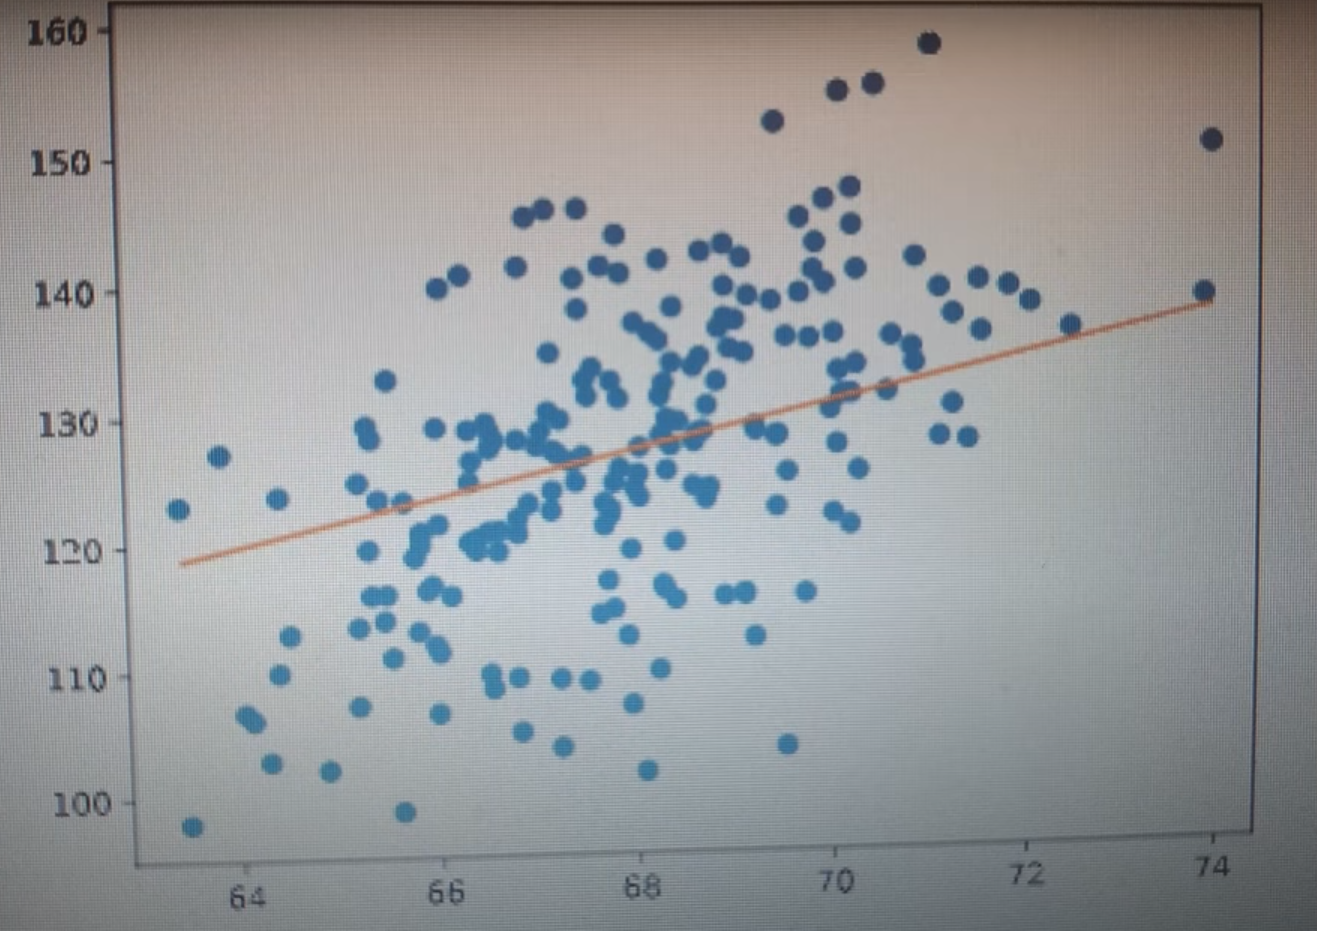
\includegraphics[width=0.04\textwidth]{latex/images/meme.PNG}
    \end{figure}

    \noindent
    Die Ausgleichsgerade wird somit durch die Steigung a = $\SI{3.3 (11)e-15}{\volt\per\ampere}$ und den y-Achsenabschnitt 
    b = $\SI{-3.5 (19)e8}{\volt\per\coulomb}$ beschrieben.
    Nach Gleichung \ref{eqn:vmax} berechnet sich das Verhätnis $\frac{\symup{h}}{\symup{e_0}}$ somit zu $\SI{2.1(7)e4}{\electronvolt}$ und die 
    Austrittsarbeit zu $\SI{2.2(12)e27}{\electronvolt}$
    \noindent

    \subsection{c)}

    \begin{figure}[H]
        \centering
        \includegraphics[width=0.85\textwidth]{build/plots/gelb.pdf}
        \caption{Die Messreihe bei \lambda = 578nm}
        \label{img:gelb}
    \end{figure}

    \noindent
    Das Diagramm beschreibt wie sich bei hohen beschleuniger Spannungen der Photostrom asymptotisch gegen einen Grenzwert annähert, im mittleren 
    Spannungsbereich ungefähr linear abfällt und nocht nicht vollständig bei der Grenzspannung $U_{\symup{g}}$ versiegt.
    Der nur asymptotisch angenäherter Photostrom ist dadurch zu erklären, dass nur begrenzt viele Elektronen bei konstanter Licht Intensität 
    durch den Photoeffekt entstehen. Diese werden in alle möglichen Richtungen verstreut, um nun alle diese Elektronen aufzufangen, auch die die sehr 
    stark aus dem Elektrischen Feld gestreut werden, wird ein sehr starkes Feld benötigt. Es werden bei hohen Spannungen auch nur noch vereinzelt
    mehr Elektronen auf die Anode geleitet, dies führt zu der asymptotischen annäherung an den Grenzwert. Somit wird der Grenzwert durch die 
    Intensität des Lichts bestimmt, um den Grenzwert bereits bei endlichen endlichen Spannungen zu erreichen müsste die Anode eine größere Fläche 
    um die Kathode am besten eine Kugelförmige Umschließung erreichen.
    Der Effekt, dass bei Erreichen der Grenzspannung kein Photostrom mehr zu sehen ist liegt hier nicht vor, da die Elektronen in der Kathode 
    bereits eine durch die Fermi-Dirac-Statistik beschriebene Energie aufweisen. Die Elektronen mit zusätzlicher Energie in Richtung der Anode 
    können somit das Gegenfeld noch überwinden und einen Photostrom erzeugen.
    Da die Photokathode bereits bei 20 Grad Celsius verdampft und somit Elektronen frei werden kann hier bereits bei kleinen Spann

    HIER FEHLT NOCH INHALT

